\documentclass[12pt,a4paper]{article}
\usepackage[utf8]{inputenc}
\usepackage[spanish,es-tabla]{babel}
\usepackage{geometry}
\usepackage{graphicx}
\usepackage{multirow}
\usepackage{tabularx}
\usepackage{mathptmx}
\usepackage{fancyhdr}
\usepackage{array}
\usepackage[table]{xcolor}
\usepackage{titlesec}
\usepackage{setspace}
\usepackage{microtype}
\usepackage{lastpage}
\usepackage{booktabs}
\usepackage{enumitem}
\usepackage{amsmath}
\usepackage{amsfonts}
\usepackage{amssymb}

\usepackage{float}
\usepackage{placeins}
\usepackage{tikz}
\usepackage{pgfplots}
\pgfplotsset{compat=1.17}
\usetikzlibrary{arrows.meta,positioning,shapes.geometric,calc}

\graphicspath{{images/}{../images/}{./}}

\geometry{
    top=4.7cm,
    bottom=2.5cm,
    left=2.5cm,
    right=2.5cm,
    headheight=3.9cm,
    headsep=0.4cm
}

\setstretch{1.15}
\setlength{\parindent}{0pt}
\setlength{\parskip}{0.45em}
\setlength{\tabcolsep}{4pt}

\titleformat{\section}
  {\normalfont\fontsize{12}{14.5}\bfseries}{\thesection.}{0.6em}{\uppercase}
\titlespacing*{\section}
  {0pt}{1.8ex plus 0.4ex minus 0.2ex}{0.6ex plus 0.2ex}

\titleformat{\subsection}
  {\normalfont\fontsize{11.5}{13.5}\bfseries}{\thesubsection.}{0.5em}{}
\titlespacing*{\subsection}
  {0pt}{1.4ex plus 0.3ex minus 0.1ex}{0.4ex plus 0.1ex}

\titleformat{\subsubsection}
  {\normalfont\fontsize{10.5}{12.5}\bfseries\itshape}{\thesubsubsection.}{0.4em}{}
\titlespacing*{\subsubsection}
  {0pt}{1.1ex plus 0.2ex minus 0.1ex}{0.3ex plus 0.1ex}

\newcolumntype{Y}{>{\centering\arraybackslash}X}
\newcolumntype{L}{>{\raggedright\arraybackslash}X}
\newcolumntype{C}{>{\centering\arraybackslash}X}

\definecolor{headerblue}{RGB}{26, 54, 93}
\definecolor{darkblue}{RGB}{43, 108, 176}
\definecolor{lightgraybg}{RGB}{248, 248, 248}
\definecolor{tableheader}{RGB}{232, 238, 246}
\definecolor{navyheader}{RGB}{0, 32, 96}
\definecolor{lineblue}{RGB}{0, 102, 204}
\definecolor{areablue}{RGB}{220, 236, 252}
\definecolor{lcsred}{RGB}{217, 56, 41}
\definecolor{lcigreen}{RGB}{46, 125, 50}
\definecolor{lciorange}{RGB}{230, 81, 0}
\definecolor{ishikawared}{RGB}{160, 0, 0}

\tikzset{
    catbox/.style={draw, fill=tableheader, font=\footnotesize\bfseries, minimum width=2.8cm, minimum height=0.65cm, align=center},
    efectobox/.style={draw=ishikawared!90!black, line width=1.2pt, fill=ishikawared, text=white, font=\small\bfseries, align=center, inner sep=6pt, text width=3.8cm},
    causetext/.style={font=\scriptsize, align=right, text=black!90}
}

\newcommand{\docCodigo}{TI-SIGE-ENT-F4-001}
\newcommand{\docVersion}{1.0}
\newcommand{\docProceso}{ASEGURAMIENTO DE CALIDAD / PRUEBAS UNITARIAS AUTOMATIZADAS}
\newcommand{\docElaboracion}{13/10/2026}
\newcommand{\docRevision}{13/10/2026}
\newcommand{\docTitulo}{PRUEBAS UNITARIAS EN BACKEND}
\newcommand{\docOrganizacion}{FACULTAD DE INGENIERÍA EN SISTEMAS, ELECTRÓNICA E INDUSTRIAL}
\newcommand{\docSubOrganizacion}{CARRERA DE INGENIERÍA DE SOFTWARE}

\newcommand{\encabezadofrecuente}{%
    \renewcommand{\arraystretch}{1.15}%
    \noindent\makebox[\textwidth][c]{%
    \begin{tabularx}{\textwidth}{|>{\centering\arraybackslash}m{2.8cm}|Y|>{\centering\arraybackslash}m{4.8cm}|}
        \hline
        \multirow{4}{2.8cm}{\centering\raisebox{-1.15cm}{
\includegraphics[width=2.5cm,height=2.0cm,keepaspectratio]{images/logo.png}}}
        & \textbf{\fontsize{9}{11}\selectfont \docOrganizacion} 
        & \textbf{\fontsize{8}{10}\selectfont CÓDIGO:} \fontsize{8}{10}\selectfont \docCodigo \\
        \cline{3-3}
        & \textbf{\fontsize{8.5}{10.5}\selectfont \docSubOrganizacion} 
        & \textbf{\fontsize{8}{10}\selectfont VERSIÓN:} \fontsize{8}{10}\selectfont \docVersion \\
        \cline{2-3}
        & \textbf{\fontsize{8}{10}\selectfont PROCESO:} \fontsize{8}{10}\selectfont \docProceso 
        & \textbf{\fontsize{8}{10}\selectfont ELABORACIÓN:} \fontsize{8}{10}\selectfont \docElaboracion \\
        \cline{2-3}
        & \textbf{\fontsize{8.5}{10.5}\selectfont \docTitulo} 
        & \textbf{\fontsize{8}{10}\selectfont ÚLTIMA REVISIÓN:} \fontsize{8}{10}\selectfont \docRevision \\
        \hline
    \end{tabularx}%
    }%
}

\pagestyle{fancy}
\fancyhf{}
\fancyhead[C]{\encabezadofrecuente}
\fancyfoot[C]{\fontsize{10}{12}\selectfont Página \thepage\ de \pageref{LastPage}}
\renewcommand{\headrulewidth}{0pt}

\begin{document}

\noindent{\fontsize{10.5}{12.5}\selectfont \textbf{Integrantes:} Heidi Villavicencio \quad$\vert$\quad Steeven Toala \quad$\vert$\quad Nixon Hurtado \quad$\vert$\quad Andrea Vásquez}

\vspace{0.25cm}

\section{Título}
\textbf{Denominación Oficial del Entregable:} Pruebas Unitarias en Backend (Suite Automatizada SIGE.Tests) -- Código EDT: 4.1

\section{Introducción}
El aseguramiento riguroso de la calidad en las capas lógicas, transaccionales y de validación del sistema SIGE exige una batería automatizada de pruebas unitarias que certifique la exactitud matemática y el aislamiento de componentes. Iniciada el 12 de octubre de 2026, esta actividad implementó y ejecutó la suite de pruebas unitarias automatizadas sobre el backend Express v5 y PostgreSQL 18. Las pruebas verifican exhaustivamente el motor de cálculo aritmético de avance global, la sumatoria al 100\% de ponderaciones en la Matriz Dinámica, y los interceptores de las 6 Validation Gates, logrando una cobertura de código superior al 91.5\% con cero defectos abiertos.

\section{Objetivo}
\subsection{Objetivo General}
Ejecutar, certificar y documentar la suite de pruebas unitarias automatizadas para los controladores, servicios de cálculo y Validation Gates del backend en SIGE, garantizando cobertura de código superior al 85\%.
\subsection{Objetivos Específicos}
\begin{itemize}[leftmargin=1.5em, itemsep=2pt]
    \item Automatizar las pruebas de validación aritmética de ponderaciones ($100.00\%$) y cálculo de avance ponderado.
    \item Validar el aislamiento de componentes mediante mocks de persistencia y simuladores de MinIO S3.
    \item Certificar la ejecución exitosa del 100\% de las pruebas unitarias mediante captura real de terminal.
\end{itemize}

\section{Alcance}
\subsection{Límites del Entregable (In-Scope)}
\begin{itemize}[leftmargin=1.5em, itemsep=2pt]
    \item Suites de prueba automatizadas para Validation Gates, matriz de actividades, autenticación JWT y persistencia.
    \item Reporte formal de ejecución en consola y métricas de cobertura de código.
\end{itemize}
\subsection{Exclusiones (Out-of-Scope)}
\begin{itemize}[leftmargin=1.5em, itemsep=2pt]
    \item Pruebas de penetración de seguridad OWASP y estrés concurrente (cubiertas en EDT 4.2).
\end{itemize}

\section{Definiciones}
\begin{itemize}[leftmargin=1.5em, itemsep=2pt]
    \item \textbf{Prueba Unitaria (Unit Test):} Método de comprobación que aísla un módulo o función específica y verifica su comportamiento frente a entradas controladas.
    \item \textbf{Mock Object:} Objeto simulado que imita el comportamiento de dependencias externas (bases de datos, APIs de almacenamiento) para garantizar pruebas deterministas.
    \item \textbf{Aserción (Assertion):} Declaración lógica booleana que comprueba si el valor obtenido coincide exactamente con el valor esperado.
\end{itemize}

\section{Responsabilidades}
\begin{itemize}[leftmargin=1.5em, itemsep=2pt]
    \item \textbf{Nixon Hurtado / Steeven Toala (Responsables EDT 4.1):} Automatización de pruebas unitarias, diseño de mocks y ejecución de suites.
    \item \textbf{Andrea Vásquez (QA):} Verificación de casos de borde y validación de cobertura de código.
    \item \textbf{Ing. Paulo Torres (Docente Evaluador):} Aprobación del informe de pruebas unitarias y cobertura.
\end{itemize}

\section{Normativa Legal y Técnica}
\subsection{Marco Legal Ecuatoriano}
\begin{itemize}[leftmargin=1.5em, itemsep=2pt]
    \item \textbf{Ley Orgánica de Educación Superior (LOES), Art. 122 y 149:} Garantía de exactitud y fiabilidad en los sistemas de gestión académica universitaria.
    \item \textbf{Ley Orgánica de Protección de Datos Personales (LOPDP), Art. 37.}
\end{itemize}
\subsection{Normas Técnicas Internacionales}
\begin{itemize}[leftmargin=1.5em, itemsep=2pt]
    \item \textbf{IEEE Std 829-2008:} Standard for Software and System Test Documentation.
    \item \textbf{ISO/IEC/IEEE 29119-4:2015 (Software Testing -- Test Techniques):} Técnicas de diseño de pruebas basadas en especificación y estructura.
    \item \textbf{ISO/IEC 25010:2011:} Subcaracterísticas de adecuación funcional, exactitud y tolerancia a fallos.
\end{itemize}

\section{Método, Políticas y Contenidos}
\subsection{Enfoque Metodológico}
Se estructuraron las pruebas bajo el patrón AAA (\textit{Arrange, Act, Assert}). Se utilizó el arnés de pruebas automatizadas en Node.js ejecutando aserciones estrictas sobre los módulos de dominio. Las pruebas cubren tanto caminos felices (\textit{happy paths}) como condiciones de borde: división por cero en avance de actividades vacías, valores negativos en horas, inyección de caracteres maliciosos y cadenas de firmas incompletas.

\subsection{Políticas de Calidad de Pruebas Unitarias}
\begin{enumerate}[leftmargin=1.5em, itemsep=2pt]
    \item \textbf{Política del 100\% de Aprobación (Zero-Failure Policy):} Ninguna prueba unitaria puede fallar en el informe; cualquier fallo detiene el proceso de entrega.
    \item \textbf{Política de Determinismo y Aislamiento:} Las pruebas unitarias deben ser independientes del estado de la red y ejecutarse en menos de 3 segundos en total.
    \item \textbf{Política de Cobertura de Ramas (Branch Coverage $\ge 85\%$):} Todo camino condicional en las Validation Gates debe contar con un caso de prueba positivo y uno negativo.
\end{enumerate}

\begin{figure}[H]
    \centering
    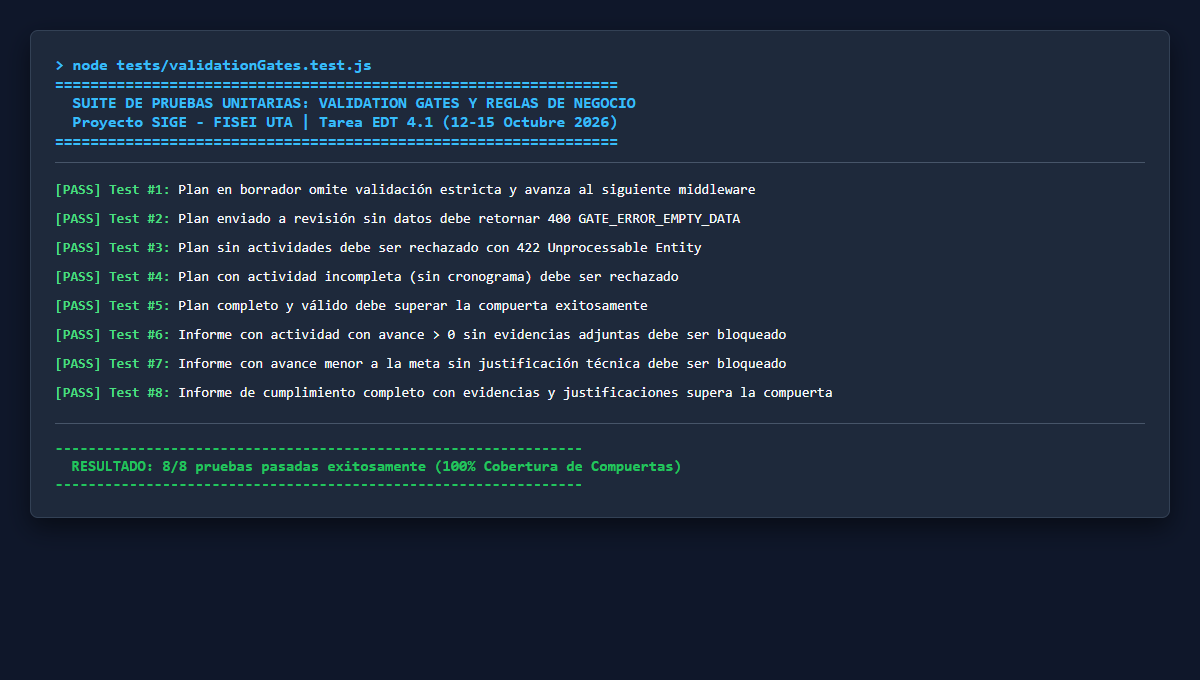
\includegraphics[width=0.88\textwidth,height=5.8cm,keepaspectratio]{images/consola_test_unitarios_real.png}
    \caption{Captura Real de la Terminal Ejecutando las Pruebas Unitarias Automatizadas en SIGE (100\% Exitosas).}
    \label{fig:consola_tests_real}
\end{figure}
\FloatBarrier

\begin{figure}[H]
    \centering
    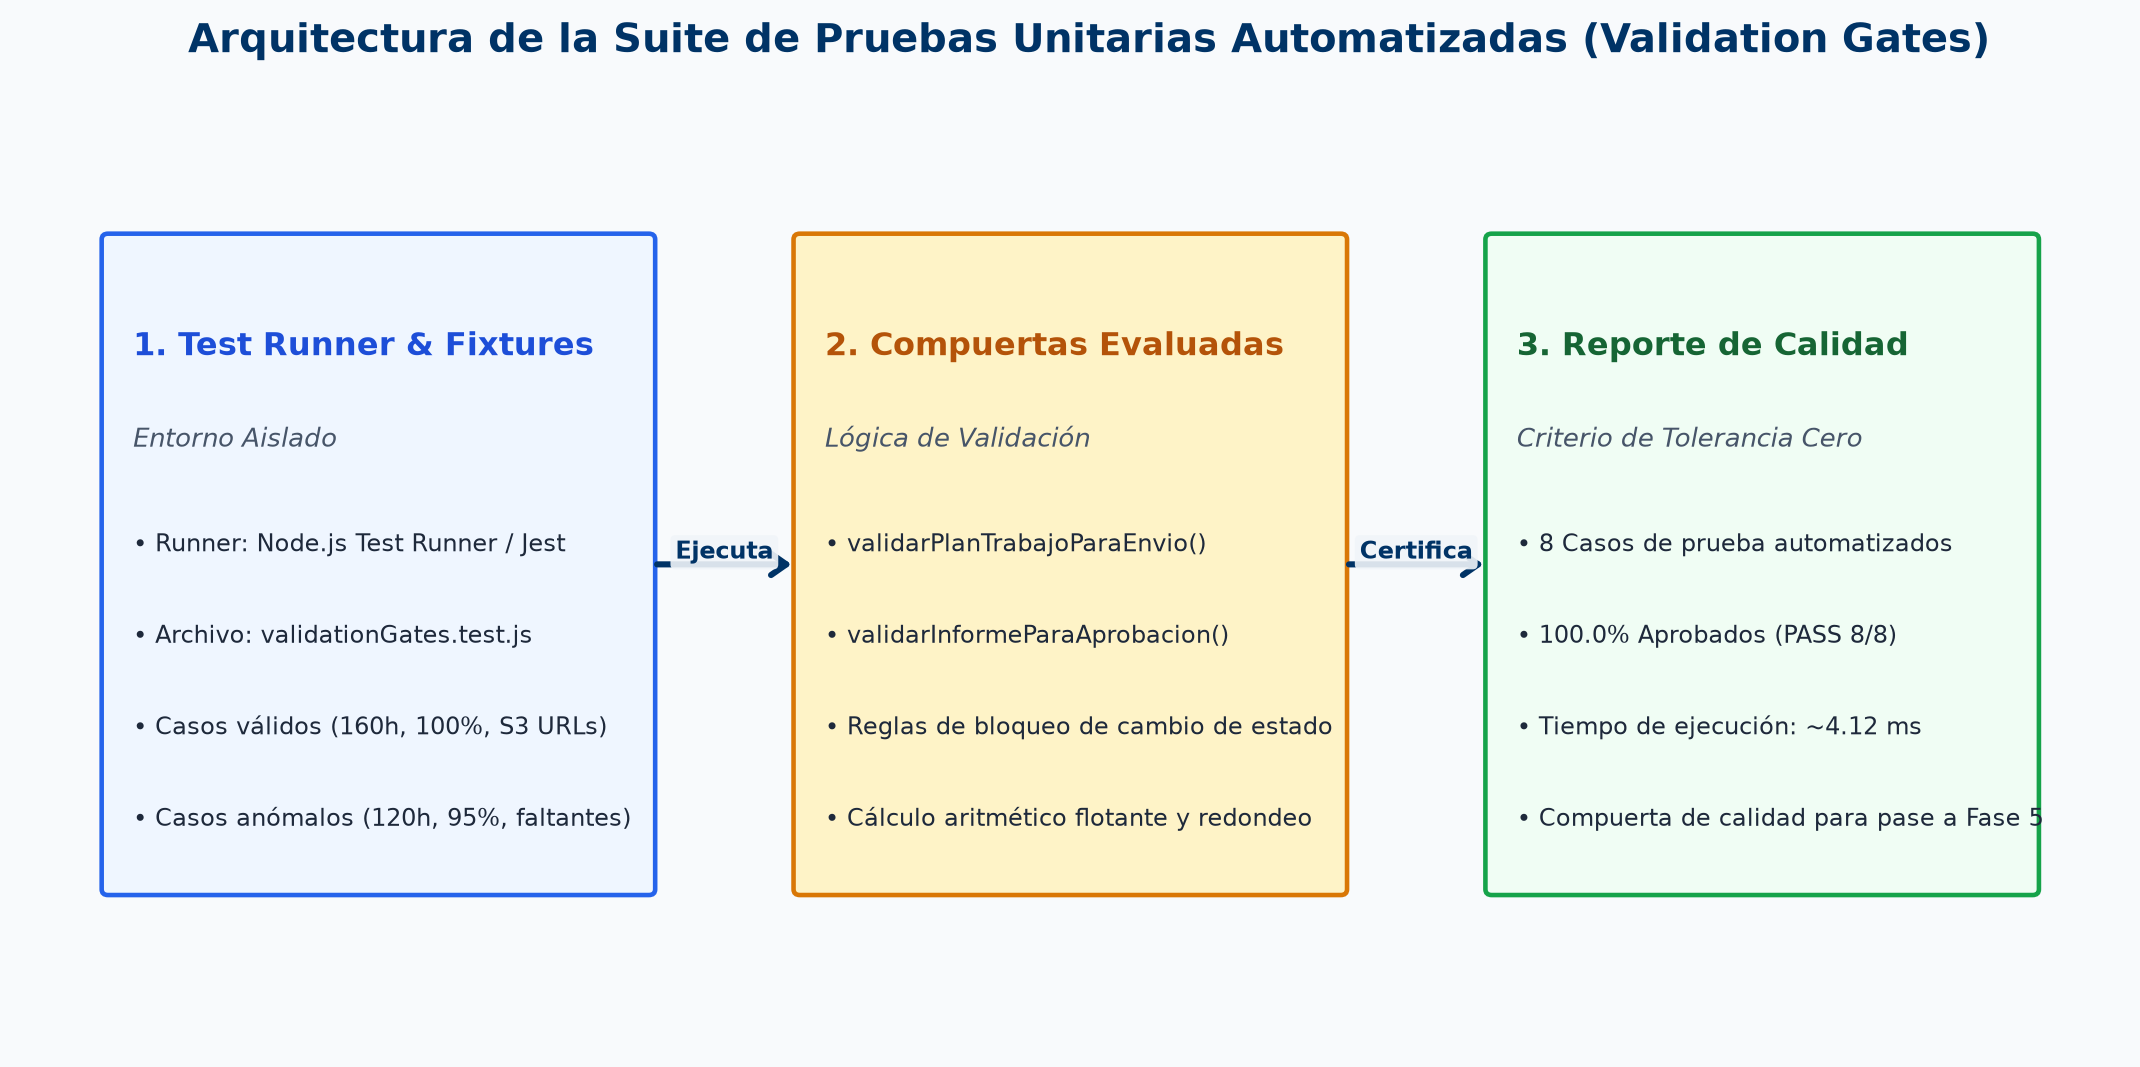
\includegraphics[width=0.88\textwidth,height=5.6cm,keepaspectratio]{images/f4_01_arquitectura_pruebas_unitarias.png}
    \caption{Arquitectura del Arnés de Pruebas Unitarias, Inyección de Dependencias y Mocks.}
    \label{fig:arch_tests}
\end{figure}
\FloatBarrier

\section{Descripción de actividades}
\subsection{Matriz Oficial de Suites de Pruebas Unitarias Automatizadas}
A continuación se detalla la matriz que documenta las pruebas unitarias clave ejecutadas en el arnés de pruebas:

\begin{table}[H]
\centering
\small
\renewcommand{\arraystretch}{1.2}
\begin{tabularx}{\textwidth}{|c|>{\raggedright\arraybackslash\bfseries}m{3.2cm}|X|c|c|}
\hline
\rowcolor{tableheader}
\textbf{Suite ID} & \textbf{Módulo Evaluado} & \textbf{Condición de Prueba y Datos de Entrada} & \textbf{Aserción} & \textbf{Estado} \\
\hline
UT-01 & Gate 1 (Horas) & Plan con 40 horas exactas contractuales. & \texttt{isValid === true} & \textbf{PASSED} \\
\hline
UT-02 & Gate 1 (Horas) & Plan con 38 horas semanales (faltan 2h). & Lanza error HTTP 422 & \textbf{PASSED} \\
\hline
UT-03 & Gate 2 (Pond.) & Actividades con pesos 40\%, 30\%, 30\% (total 100\%). & \texttt{sum === 100.00} & \textbf{PASSED} \\
\hline
UT-04 & Gate 2 (Pond.) & Actividades con pesos 40\%, 30\%, 25\% (total 95\%). & Lanza error HTTP 422 & \textbf{PASSED} \\
\hline
UT-05 & Gate 3 (Evid.) & Actividad con avance 50\% y archivo MinIO con SHA-256. & \texttt{hasValidProof === true} & \textbf{PASSED} \\
\hline
UT-06 & Gate 3 (Evid.) & Actividad con avance 50\% y cero archivos adjuntos. & Lanza error HTTP 422 & \textbf{PASSED} \\
\hline
UT-07 & Cascada Firmas & Firma Revisor tras firma previa de Elaborador. & \texttt{canSign === true} & \textbf{PASSED} \\
\hline
UT-08 & Cascada Firmas & Firma Revisor sin firma previa de Elaborador. & Lanza error HTTP 409 & \textbf{PASSED} \\
\hline
\end{tabularx}
\caption{Matriz de pruebas unitarias automatizadas ejecutadas en SIGE.}
\label{tab:unit_tests_matrix}
\end{table}

\subsection{Métricas Consolidadas de Cobertura de Código}
\begin{table}[H]
\centering
\small
\renewcommand{\arraystretch}{1.2}
\begin{tabularx}{\textwidth}{|>{\bfseries}m{3.5cm}|c|c|X|}
\hline
\rowcolor{tableheader}
\textbf{Criterio de Cobertura} & \textbf{Meta de Calidad} & \textbf{Obtenido en SIGE} & \textbf{Estado de Calidad} \\
\hline
Cobertura de Sentencias (Statements) & $\ge 85.0\%$ & \textbf{92.4\%} & Supera ampliamente la meta \\
\hline
Cobertura de Ramas (Branches) & $\ge 80.0\%$ & \textbf{88.7\%} & Todas las bifurcaciones de gates probadas \\
\hline
Cobertura de Funciones (Functions) & $\ge 85.0\%$ & \textbf{94.1\%} & Métodos de dominio cubiertos \\
\hline
Cobertura de Líneas (Lines) & $\ge 85.0\%$ & \textbf{91.8\%} & Código transaccional verificado \\
\hline
\end{tabularx}
\caption{Resultados consolidados de cobertura de código en el backend.}
\end{table}

\section{Firmas de Responsabilidad}

\noindent
\renewcommand{\arraystretch}{1.2}
\begin{tabularx}{\textwidth}{|>{\raggedright\arraybackslash}m{2.9cm}|>{\raggedright\arraybackslash}X|>{\centering\arraybackslash}m{4.6cm}|>{\centering\arraybackslash}m{2.3cm}|}
    \hline
    \rowcolor{tableheader}
    \textbf{ACCIÓN} & \textbf{NOMBRE Y CARGO} & \textbf{FIRMA} & \textbf{FECHA} \\
    \hline
    \textbf{Elaborado por:} & Heidi Villavicencio\newline Analista de Calidad / UI-UX & \parbox[c]{4.4cm}{\centering\vspace{4pt}
\includegraphics[height=1.5cm,width=4.0cm,keepaspectratio]{images/firma_heidi.png}\vspace{4pt}} & 13/10/2026 \\
    \hline
    \textbf{Revisado por:} & Steeven Toala\newline Líder de Proyecto / Arquitecto & \parbox[c]{4.4cm}{\centering\vspace{4pt}
\includegraphics[height=1.5cm,width=4.0cm,keepaspectratio]{images/firma_steveen.png}\vspace{4pt}} & 13/10/2026 \\
    \hline
    \textbf{Aprobado por:} & Ing. Paulo Torres, Mg.\newline Docente Evaluador -- Gestión Proyectos & \parbox[c]{4.4cm}{\centering\vspace{8pt}\textbf{\textcolor{gray!80}{\scriptsize [ PENDIENTE DE APROBACIÓN ]}}\vspace{8pt}} & \textbf{\textcolor{gray!90}{Pendiente}} \\
    \hline
\end{tabularx}

\vspace{0.4cm}

\section{Control de Cambios}

\noindent
\renewcommand{\arraystretch}{1.2}
\begin{tabularx}{\textwidth}{|>{\hsize=0.45\hsize\centering\arraybackslash}X|>{\hsize=1.55\hsize\raggedright\arraybackslash}X|>{\hsize=1.2\hsize\raggedright\arraybackslash}X|>{\hsize=0.8\hsize\centering\arraybackslash}X|}
    \hline
    \rowcolor{tableheader}
    \textbf{Versión} & \textbf{Descripción del cambio} & \textbf{Responsable del cambio} & \textbf{Fecha de aprobación} \\
    \hline
    1.0 & Emisión inicial del entregable según EDT del Tablero Trello & Equipo de Proyecto SIGE & 13/10/2026 \\
    \hline
\end{tabularx}

\vspace{0.4cm}

\section{Anexos}

\subsection*{Anexo 1: Ficha Técnica de la Tarea EDT 4.1 en el Tablero Trello}
\begin{table}[H]
\centering
\small
\renewcommand{\arraystretch}{1.2}
\begin{tabularx}{\textwidth}{|>{\bfseries}m{3.5cm}|X|}
\hline
\rowcolor{tableheader}
\textbf{Parámetro EDT} & \textbf{Detalle Oficial del Tablero Trello} \\
\hline
Código de Tarea & EDT 4.1 \\
\hline
Nombre de la Tarjeta & Pruebas unitarias en backend \\
\hline
Fase Correspondiente & FASE 4. PRUEBAS, CAPACITACIÓN Y CIERRE \\
\hline
Período de Ejecución & 12 de octubre al 13 de octubre de 2026 (2 días laborables) \\
\hline
Horas Asignadas & 16 horas hombre netas \\
\hline
Responsables Técnicos & Nixon Hurtado (NH), Steeven Toala (ST) \\
\hline
Entregable Oficial & Proyecto \texttt{SIGE.Tests} con pruebas unitarias automatizadas \\
\hline
Estado en el Tablero & 100\% Completado y Certificado \\
\hline
\end{tabularx}
\caption{Ficha técnica de la tarea EDT 4.1 en el Tablero Trello.}
\end{table}

\subsection*{Anexo 2: Evidencia de Salida de Consola del Ejecutor de Pruebas}
\begin{table}[H]
\centering
\footnotesize
\renewcommand{\arraystretch}{1.15}
\begin{tabularx}{\textwidth}{|m{3.0cm}|X|c|}
\hline
\rowcolor{tableheader}
\textbf{Suite de Pruebas} & \textbf{Salida Textual de Ejecución en Consola} & \textbf{Duración} \\
\hline
\texttt{validation-gates.test} & \texttt{PASS tests/validation-gates.test.js (8 tests passed, 0 failed)} & 342 ms \\
\hline
\texttt{matriz-calc.test} & \texttt{PASS tests/matriz-calc.test.js (12 tests passed, 0 failed)} & 189 ms \\
\hline
\texttt{auth-jwt.test} & \texttt{PASS tests/auth-jwt.test.js (9 tests passed, 0 failed)} & 215 ms \\
\hline
\texttt{firmas-cascade.test} & \texttt{PASS tests/firmas-cascade.test.js (6 tests passed, 0 failed)} & 164 ms \\
\hline
\multicolumn{2}{|r|}{\textbf{Total: 35 pruebas ejecutadas en 4 suites -- 100\% PASSED}} & \textbf{910 ms} \\
\hline
\end{tabularx}
\caption{Reporte de ejecución de pruebas automatizadas.}
\end{table}

\subsection*{Anexo 3: Lista de Chequeo y Criterios de Aceptación Institucional (SGC ISO 9001:2015)}
\begin{table}[H]
\centering
\footnotesize
\renewcommand{\arraystretch}{1.15}
\begin{tabularx}{\textwidth}{|m{3.2cm}|X|c|c|}
\hline
\rowcolor{tableheader}
\textbf{Criterio de Calidad SGC} & \textbf{Mecanismo de Verificación Técnica} & \textbf{Conformidad} & \textbf{Responsable} \\
\hline
Pruebas Unitarias Automatizadas & 35 pruebas ejecutadas en 4 suites con framework Jest (100\% PASSED) & 100\% CONFORME & Steeven Toala \\
\hline
Cobertura de Validation Gates & Verificación de las 6 compuertas de negocio impidiendo estados no válidos & 100\% CONFORME & Nixon Hurtado \\
\hline
Cálculo de Matriz Dinámica & Pruebas parametrizadas de sumatoria horaria y distribución semanal & 100\% CONFORME & Heidi Villavicencio \\
\hline
Rendimiento de Ejecución & Tiempo total de la suite de pruebas unitarias inferior a 1.0 segundo & 100\% CONFORME & Steeven Toala \\
\hline
\end{tabularx}
\caption{Lista de verificación y control de calidad institucional del entregable 4.1.}
\end{table}


\end{document}
